\section{Procedure a supporto dei processi}


\subsection{Procedure di progetto}
\label{procedurediprogetto}

Abbiamo ritenuto poco efficiente utilizzare la piattaforma \glossario{TeamworkPM} per la gestione sia delle attività che delle modifiche, poiché l'utilizzo che volevamo farne non sfruttava appieno le funzionalità di ``Diagramma Gantt'' e ``Task List''. È stata fatta quindi la seguente separazione:
\begin{itemize}
 \item \textbf{gestione delle attività}: viene fatta utilizzando i \glossario{task} di \glossario{TeamworkPM}
 \item \textbf{gestione delle modifiche}: viene fatta utilizzando le \glossario{issue} di \glossario{GitHub}
\end{itemize}

Quando non è specificato come modificare il valore di un parametro delle \glossario{issue} bisogna mantenere il valore già presente, o quello di default se la \glossario{issue} è appena stata creata.

\subsubsection{Richiesta di modifica e segnalazione bug}
\label{aperturaissue}

\begin{figure}[H]
    \centering
    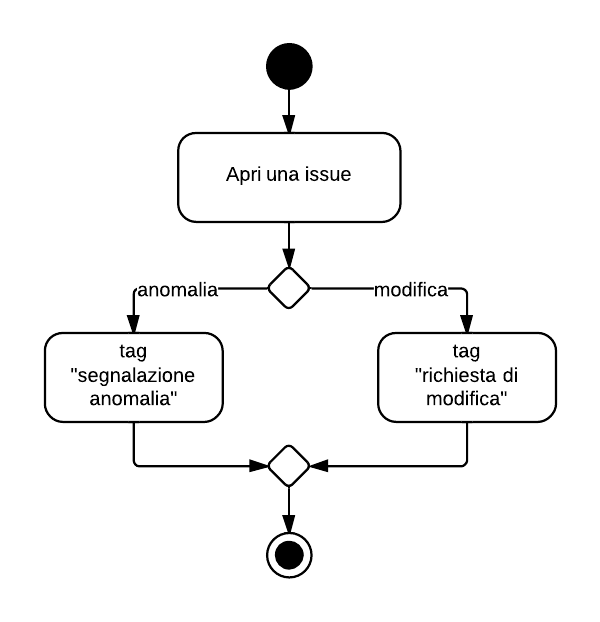
\includegraphics[width=9cm]{uml-processi/richiesta_di_modifica_e_segnalazione_bug.png}
    \caption{Richiesta di modifica e segnalazione bug}
\end{figure}

Se un membro del gruppo intende segnalare un bug o richiedere una modifica deve aprire una \glossario{issue} su \glossario{GitHub} con i seguenti parametri:
\begin{itemize}
 \item \textbf{Titolo}: un titolo breve ma descrittivo.
 \item \textbf{Descrizione}: una descrizione esaustiva dell'anomalia riscontrata o della modifica richiesta.
 \item \textbf{Tag}: uno tra i seguenti:
  \begin{itemize}
   \item \textbf{segnalazione anomalia}: da usare se si vuole segnalare un bug, un malfunzionamento, un'anomalia in genere che non dovrebbe esserci nei documenti ufficiali o nel prodotto finale;
   \item \textbf{richiesta di modifica}: da usare se si vuole richiedere al Responsabile una modifica.
  \end{itemize}
 \item \textbf{Assegnato a}: il Responsabile
 \item \textbf{Milestone}: nessuna
\end{itemize}

\subsubsection{Progettazione unità di lavoro}

\begin{figure}[H]
    \centering
    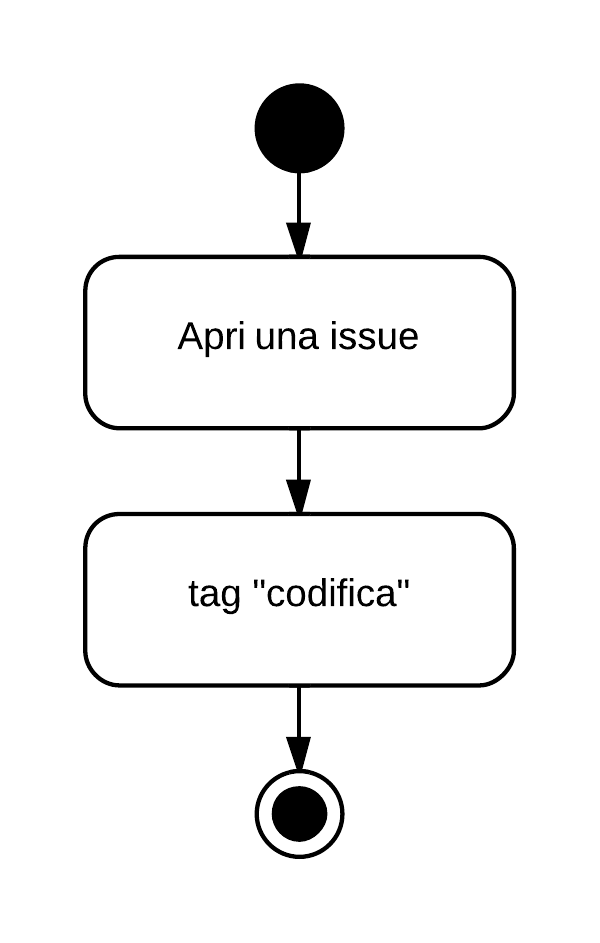
\includegraphics[height=7cm]{uml-processi/progettazione_unita_di_lavoro.png}
    \caption{Creazione compito}
\end{figure}

Il Progettista, dopo aver completata la progettazione di dettaglio, deve creare le \glossario{issue} di codifica con i seguenti parametri:
\begin{itemize}
 \item \textbf{Titolo}: un titolo breve ma descrittivo.
 \item \textbf{Descrizione}: una descrizione esaustiva dell'attività da svolgere, con tutti i riferimenti necessari.
 \item \textbf{Tag}: \textbf{codifica}
 \item \textbf{Assegnato a}: il Responsabile
 \item \textbf{Milestone}: nessuna
\end{itemize}

\subsubsection{Valutazione issue}

\begin{figure}[H]
    \centering
    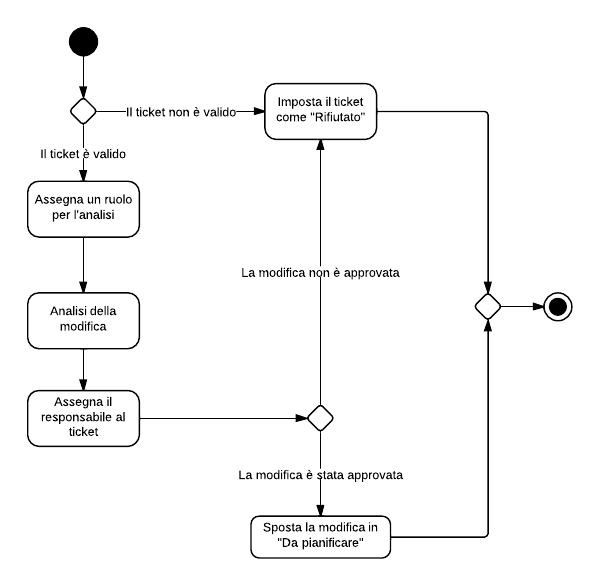
\includegraphics[width=\textwidth]{uml-processi/valutazione_issue.png}
    \caption{Valutazione issue}
\end{figure}

Il Responsabile deve valutare ogni nuova \glossario{issue}. Se ritiene che la formulazione sia corretta e se è necessario approfondire la modalità in cui verrà eseguita l'attività richiesta, allora il Responsabile deve anche assegnare la \glossario{issue} ad un ruolo competente:
\begin{itemize}
 \item \textbf{Assegnato a}: un ruolo a scelta del Responsabile
\end{itemize}

Tale ruolo, dopo averla analizzata, deve riassegnarla al Responsabile aggiungendo le informazione prodotte dall'analisi:
\begin{itemize}
 \item \textbf{Assegnato a}: il Responsabile
 \item \textbf{Descrizione}: la descrizione già presente con in aggiunta i risultati dell'analisi.
\end{itemize}

A questo punto, se il Responsabile ritiene che l'attività debba essere eseguita, pianifica la issue secondo la procedura \ref{pianificazione}.

Se il Responsabile non approva o non ritene valida la \glossario{issue} deve chiuderla impostando:
\begin{itemize}
 \item \textbf{Tag}: uno tra i seguenti
  \begin{itemize}
   \item \textbf{scritto male}: se la descrizione o il titolo sono poco comprensibili;
   \item \textbf{non lo faremo}: se ritiene che non valga la pena si svolgere l'attività richiesta;
   \item \textbf{duplicato}: se l'attività è già stata richiesta da un'altra \glossario{issue}. In questo caso è raccomandabile aggiungere nella descrizione un riferimento alla \glossario{issue} originale.
  \end{itemize}
 \item \textbf{Stato}: ``Chiuso''.
\end{itemize}

\subsubsection{Pianificazione issue}
\label{pianificazione}

\begin{figure}[H]
    \centering
    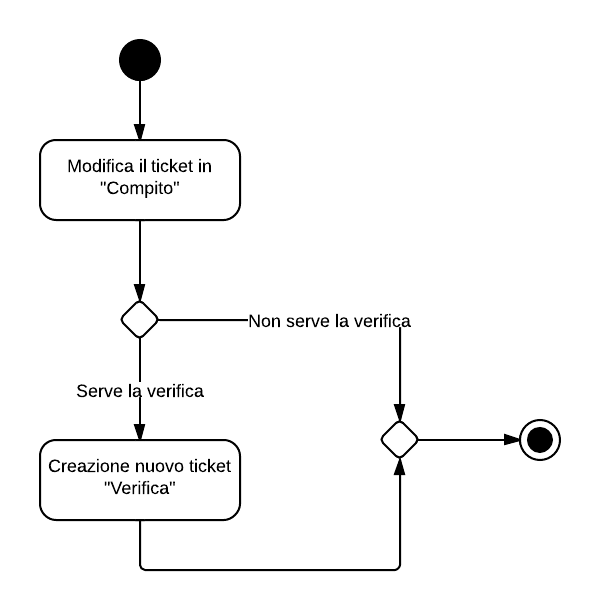
\includegraphics[width=12cm]{uml-processi/pianificazione_issue.png}
    \caption{Pianificazione issue}
\end{figure}

Il Responsabile deve pianificare le \glossario{issue} a lui assegnate e marcate ``approvato'' o ``codifica'' creando un \glossario{task}. Deve inoltre pianificare il corrispondente \glossario{task} di verifica se necessario. I \glossario{task} del compito e della modifica devono essere assegnati a persone diverse.

Modifica i parametri della \glossario{issue}:
\begin{itemize}
 \item \textbf{Assegnato a}: nessuno.
\end{itemize}

Se esiste già un \glossario{task} a cui associare la \glossario{issue} il Responsabile deve scegliere una delle seguenti opzioni:
\begin{itemize}
 \item modificare tale \glossario{task} con questi parametri:
	\begin{itemize}
		\item \textbf{Descrizione}: la descrizione precedente, con in aggiunta un riferimento evidente alla \glossario{issue}.
	\end{itemize}
 \item creare un \glossario{task} secondario (``subtask'' nel gergo di TeamworkPM) con i seguenti parametri:
	\begin{itemize}
		\item \textbf{Titolo}: un titolo breve ma descrittivo, magari simile a quello della \glossario{issue}.
		\item \textbf{Descrizione}: una breve descrizione, con un riferimento evidente alla \glossario{issue}.
		\item \textbf{Assegnato a}: la stessa persona a cui è associato il \glossario{task} principale.
	\end{itemize}
\end{itemize}

Se il \glossario{task} non esiste, allora deve crearne uno nuovo seguendo la procedura \ref{creazionetask}.

Analogamente, se esiste già un \glossario{task} a cui associare la verifica, il Responsabile deve scegliere una delle seguenti opzioni:
\begin{itemize}
 \item modificare tale \glossario{task} di verifica con questi parametri:
	\begin{itemize}
		\item \textbf{Descrizione}: la descrizione precedente, con in aggiunta un riferimento evidente al \glossario{task} da verificare.
	\end{itemize}
 \item creare un \glossario{task} secondario (``subtask'' nel gergo di TeamworkPM) con i seguenti parametri:
	\begin{itemize}
		\item \textbf{Titolo}: un titolo breve ma descrittivo, magari simile a quello della \glossario{issue}.
		\item \textbf{Descrizione}: una breve descrizione, con un riferimento evidente alla \glossario{issue}.
		\item \textbf{Assegnato a}: la stessa persona a cui è associato il \glossario{task} principale.
	\end{itemize}
\end{itemize}

Se il \glossario{task} di verifica non esiste, allora deve crearne uno nuovo seguendo la procedura \ref{creazionetask}.

\subsubsection{Creazione task}
\label{creazionetask}

\begin{figure}[H]
    \centering
    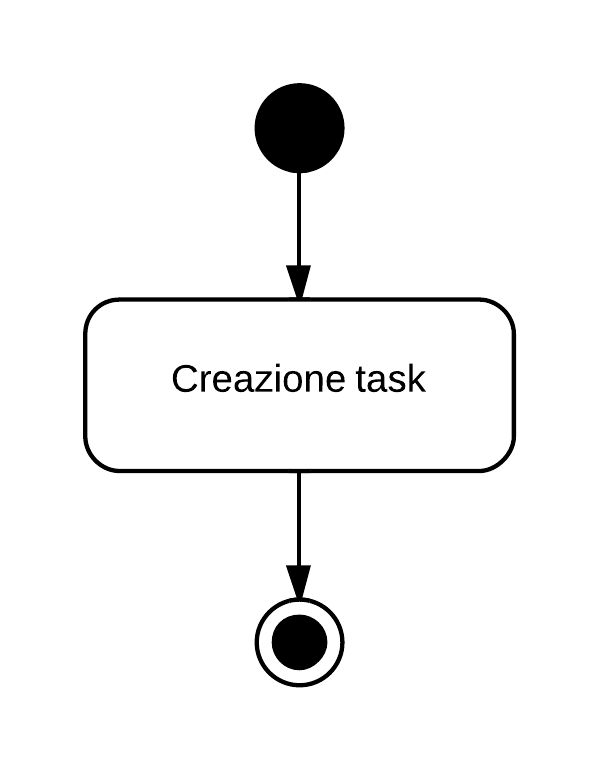
\includegraphics[height=6cm]{uml-processi/creazione_task.png}
    \caption{Creazione task}
\end{figure}

Il Responsabile può creare \glossario{task} con i seguenti parametri:
\begin{itemize}
 \item \textbf{Titolo}: il titolo dell'attività nel formato ``\{identificativo\} - \{titolo\} (\{ruolo\})'', dove
	\begin{itemize}
		\item \textbf{identificativo}: il codice che identifica l'attività nel \emph{Piano di progetto}, se presente;
		\item \textbf{titolo}: il titolo, breve e descrittivo, dell'attività.
		\item \textbf{ruolo}: il ruolo a cui è assegnato il \glossario{task}
	\end{itemize}
 \item \textbf{Assegnato a}: un membro del gruppo a scelta del Responsabile.
 \item \textbf{Pianificazione}: a scelta del Responsabile.
 \item \textbf{Descrizione}: una descrizione dell'attività (raccomandata).
 \item \textbf{Dipendenze}: i \glossario{task} di cui bisogna attendere il termine prima di poter svolgere questo \glossario{task}. In particolare, i \glossario{task} di verifica devono sempre dipendere dai \glossario{task} che devono verificare.
\end{itemize}

Solo il Responsabile può creare nuovi task.

\subsubsection{Esecuzione compito}

\begin{figure}[H]
    \centering
    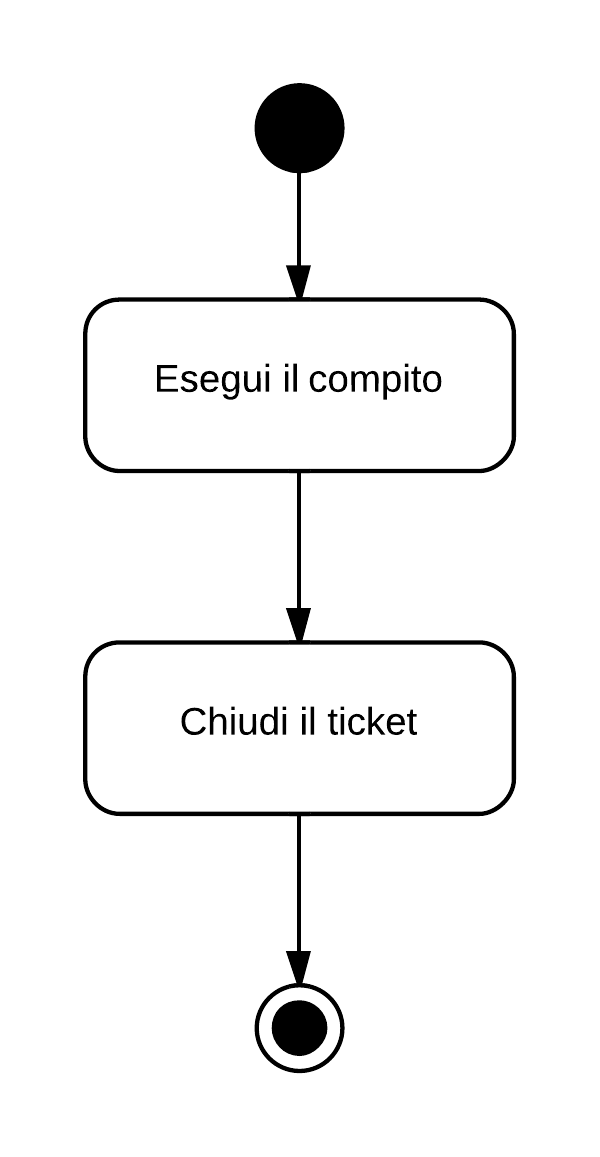
\includegraphics[width=11cm]{uml-processi/esecuzione_compito.png}
    \caption{Esecuzione compito}
\end{figure}

Il ruolo a cui è assegnato un \glossario{task} non di verifica, dopo aver svolto l'attività richiesta, deve chiudere il \glossario{task}:
\begin{itemize}
 \item \textbf{Stato task}: ``Chiuso''.
\end{itemize}

Inoltre deve chiudere ogni eventuale \glossario{issue} aperta associata:
\begin{itemize}
 \item \textbf{Stato issue}: ``Chiuso''.
\end{itemize}

\subsubsection{Esecuzione verifica}

\begin{figure}[H]
    \centering
    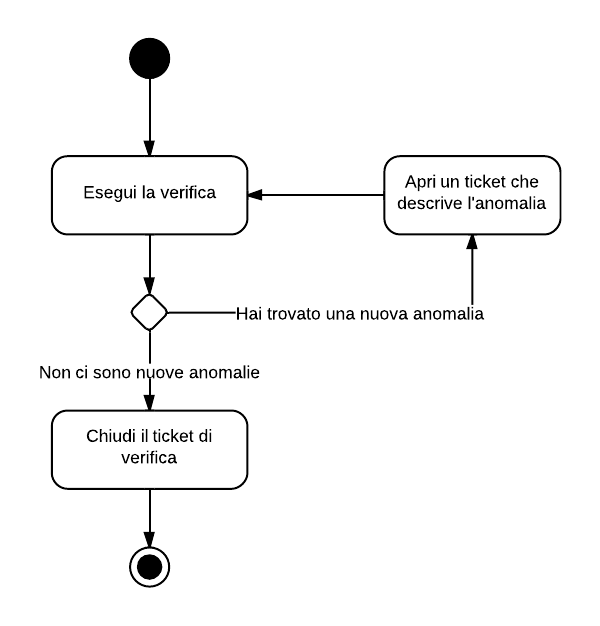
\includegraphics[width=10cm]{uml-processi/esecuzione_verifica.png}
    \caption{Esecuzione verifica}
\end{figure}

Il verificatore a cui è assegnato un \glossario{task}, dopo aver svolto l'attività richiesta, deve chiudere il \glossario{task}:
\begin{itemize}
 \item \textbf{Stato}: ``Chiuso''.
\end{itemize}

Nel caso in cui il verificatore trovi bug o non conformità significative deve creare una \glossario{issue}, seguendo la procedura descritta nella sezione \ref{aperturaissue}.

\subsection{Pianificazione}

Come convenzione il gruppo ha scelto una soglia oraria giornaliera e settimanale in cui lavorare al progetto:
		
		\begin{itemize}
			\item L'orario di lavoro giornaliero è da considerarsi dalle 9:00 alle 12:00 e dalle 13:00 alle 17:00, per un massimo di 7 ore;
			\item I giorni lavorativi settimanali sono dal Lunedì al Venerdì.
		\end{itemize}
		
		Le ore impiegate oltre queste soglie sono considerate ore di \textbf{straordinario}. In particolare al Responsabile è raccomandato pianificare due ore di lavoro al giorno, per un totale di 10 ore settimanali.
		
		Il responsabile nell'assegnare task terrà conto di quanto inserito nel calendario, come indicato nel capitolo \ref{Calendario condiviso}, e di quanto indicato nel capitolo \ref{rotazioneruoli} riguardo la rotazione dei ruoli. 
		

\subsection{Analisi dei requisiti}

Dal capitolato e dagli incontri con il proponente gli Analisti dovranno estrarre i requisiti del progetto, producendo l'Analisi dei Requisiti.

Tutti i requisiti che si possono evincere dal capitolato o ad un incontro con il proponente vanno specificati nell'Analisi dei Requisiti.

Per agevolare l'analisi dei requisiti viene utilizzata la tecnica dei casi d'uso.

    \subsubsection{Tracciamento requisiti}
     I requisiti vengono tracciati mediante il software \emph{Requisteak} appositamente creato dal gruppo \GroupName{}. Tale strumento è raggiungibile all'indirizzo:
     \begin{center}
         \url{http://steakholders.herokuapp.com}.
     \end{center} 
     Le credenziali di accesso sono le seguenti:
     \begin{itemize}
        \item \textbf{Username}: \texttt{committente@steakholders.com};
        \item \textbf{Password}: \texttt{unipd2013}.
     \end{itemize}
     
\subsubsection{Casi d'Uso}

Ogni caso d'uso dovrà presentare i seguenti campi:
\begin{itemize}
 \item Codice identificativo
 \item Titolo
 \item Diagramma UML
 \item Attori primari
 \item Attori secondari 
 \item Scopo e descrizione
 \item Precondizione
 \item Postcondizione
 \item Flusso principale degli eventi
 \item Scenari alternativi
\end{itemize}

\subsubsection{Codice identificativo}

Ogni caso d'uso è identificato da un codice, che segue il seguente formalismo:
\begin{center}
    \code{UC\{X\} \{Gerarchia\}}
\end{center}

Dove:
\begin{itemize}
 \item \textbf{X} corrisponde all'ambito di riferimento e può assumere i seguenti valori:
    \begin{itemize}
     \item[] \textbf{U} = Ambito \glossario{Utente};
     \item[] \textbf{S} = Ambito \glossario{Sviluppatore}.
    \end{itemize}

     \item \textbf{Gerarchia} identifica la relazione gerarchica che c'è tra i casi d'uso di uno stesso ambito. C'è quindi una struttura gerarchica per ogni ambito dei casi d'uso. La numerazione potrebbe non essere continua nel caso in cui vengano rimossi alcuni degli use case numerati in precedenza.
\end{itemize}

\subsubsection{Requisiti}

Ogni requisito dovrà presentare i seguenti campi:
\begin{itemize}
 \item Codice identificativo
 \item Descrizione
 \item Fonti
\end{itemize}

\subsubsection{Codice identificativo}

Ogni requisito è identificato da un codice, che segue il seguente formalismo:
\begin{center}
    \code{R\{X\}\{Y\}\{Z\} \{Gerarchia\}}
\end{center}

Dove:
\begin{itemize}
 \item \textbf{X} corrisponde al sistema di riferimento e può assumere i seguenti valori:
    \begin{itemize}
     \item[] \textbf{A} = Applicazione \glossario{Maap};
     \item[] \textbf{F} = \glossario{Framework} di \glossario{Maap};
     \item[] \textbf{S} = \glossario{Maas}.
    \end{itemize}

 \item \textbf{Y} corrisponde alla tipologia del requisito e può assumere i seguenti valori:
    \begin{itemize}
     \item[] \textbf{1} = Funzionale;
     \item[] \textbf{2} = Di prestazione;
     \item[] \textbf{3} = Di qualità;
     \item[] \textbf{4} = Vincolo.
    \end{itemize}

 \item \textbf{Z} corrisponde alla priorità del requisito e può assumere i seguenti valori:
    \begin{itemize}
     \item[] \textbf{O} = Obbligatorio
     \item[] \textbf{D} = Desiderabile
     \item[] \textbf{F} = Facoltativo o opzionale
    \end{itemize}

 \item \textbf{Gerarchia} identifica la relazione gerarchica che c'è tra i requisiti di uno stesso tipo. C'è quindi una struttura gerarchica per ogni tipologia di requisito.
\end{itemize}

\subsubsection{UML}

Per i diagrammi deve essere utilizzata il linguaggio \emph{UML versione 2.0}.


\subsection{Progettazione}
%\subsubsection{Specifica Tecnica}
La progettazione deve dimostrabilmente rispettare tutti i requisiti che il gruppo ha concordato con il committente. In particolare i componenti progettati devono essere tracciabili rispetto al requisito che soddisfano.
Di seguito vengono elencate le norme a carico dei \emph{Progettisti}.

    \subsubsection{Diagrammi UML}
    Si dovrà usare il linguaggio \glossario{UML} \emph{versione 2.0} per i seguenti diagrammi:
\begin{itemize}
 \item \textbf{Diagrammi dei package:} dovranno essere presenti sia per l'architettura generale che di dettaglio, sarà fondamentale per definire i moduli all'interno del \glossario{framework} \glossario{Node.js} richiesto dal capitolato;
 \item \textbf{Diagrammi delle classi:} qualora il progetto utilizzasse delle classi, i diagrammi delle classi dovranno essere presenti sia per l'architettura generale che di dettaglio. Nell'ambiente \glossario{Node.js} a prima vista sembra che siano poco utilizzate, a favore dei \glossario{package};
 \item \textbf{Diagrammi di flusso:} qualora la codifica di un'unità del progetto sia particolarmente complessa, dovrà essere presente il relativo diagramma di flusso che il programmatore dovrà seguire;
\end{itemize}

    \subsubsection{Stile di progettazione}
    \begin{itemize}
        \item La progettazione dovrà usare quanto più possibile \glossario{design pattern} globalmente affermati, la loro scelta dovrà essere giustificata;
        \item Suddividere il progetto in \glossario{moduli}, in accordo con lo stile di progettazione dell'ambiente \glossario{Node.js};
        \item Non utilizzare codice sincrono per operazioni di \glossario{I/O};
        \item Limitare quanto più possibile le \glossario{callback} annidate;
    \end{itemize}


    %\paragraph{Test di integrazione}
    %I test di integrazione avvengono mediante la definizione e l'utilizzo di opportuni strumenti di test per verificare che i componenti del sistema funzionino nella maniera prevista.


%\subsubsection{Definizione di Prodotto}
%La \emph{Definizione di Prodotto} è la descrizione dettagliata della progettazione descritta nella \emph{Specifica Tecnica}. Questo documento rappresenta lo stadio avanzato della progettazione e indicherà ogni singolo componente del sistema permettendo ai \emph{Programmatori} di procedere con lo sviluppo. Parallelamente alla progettazione di dettaglio dovranno essere progettati i relativi test di unità che verranno descritti nel \PianoDiQualifica .

%   \paragraph{Definizione di classe}
%   Le classi progettate devono comparire nella \emph{Definizione di Prodotto} che dovrà descriverne l'elenco dei metodi e degli attributi, lo scopo e la funzionalità che rappresenta.
%   completare...
%   
%   % \subsubsection{Formalismo di specifica dei metodi}
%    \subsubsection{Tracciamento classi}
%   
%   \paragraph{Test di unità}
%   I \emph{Progettisti} modellano i test da effettuare sulle unità per le opportune verifiche.



%\subsubsection{Verifica della progettazione architetturale}
%\subsubsection{Verifica della progettazione di dettaglio}
%\subsubsection{Verifica del codice}
%\paragraph{Analisi Statica}
%\paragraph{Analisi Dinamica}
%\subsection{Resoconto bug}
%\subsection{Validazione output}

%\subsection{Codifica}
%   \subsubsection{Codifica e convenzioni}
%       \paragraph{Nomi}
%       \paragraph{Ricorsione}
%   \subsubsection{Documentazione}


\subsection{Codifica}

\subsubsection{Intestazione}

\begin{lstlisting}
/*
* Name: {Nome del file}
* Module: {modulo di appartenenza}
* Location: {/path/della/cartella/}
*
* History:
* Version     Date            Programmer    
* ================================================
* 1.1.3       AAAA-MM-GG      {Nome Cognome      }
* ------------------------------------------------
* ...
* {Description}
* ...
* ================================================
* 1.1.2       AAAA-MM-GG      {Nome Cognome      }
* ------------------------------------------------
* ...
*
*/
\end{lstlisting}

\begin{itemize}
 \item \textbf{Name} è il nome del file, estensione compresa.
 \item \textbf{Module} è il nome del modulo di cui il file fa parte.
 \item \textbf{Location} è il percorso del file, a partire dalla cartella principale del progetto ``/'' fino alla cartella che contiene il file. Deve iniziare e terminare con uno slash ``/".
 \item \textbf{History} è il diario delle modifiche del file. Ogni modifica è composta dai seguenti campi:
 
    \begin{itemize}
     \item \textbf{Version} è la versione del file.
     \item \textbf{Date} è la data della modifica.
     \item \textbf{Programmer} è il nome e cognome dell'autore della modifica. Al massimo può essere lungo 20 caratteri.
     \item \textbf{Description} è la spiegazione delle modifiche fatte e del motivo per cui sono state fatte.    
    \end{itemize}
\end{itemize}

\subsubsection{Formattazione}

La formattazione del codice sorgente deve essere definita in modo rigoroso e consistente, così che tutto il codice del progetto sembri che sia stato scritto da un'unica persona.

Per il codice \emph{Javascript} si è scelto di adottare le linee guida utilizzate dal progetto \emph{jQuery}, sia per l'effettiva facilità di lettura sia per la possibilità di automatizzare la formattazione del codice tramite il programma \emph{JSHint}. La pagina di riferimento è \url{http://contribute.jquery.org/style-guide/js/}.

%\paragraph{Indentazione}
%\subsubsection{Norme di validazione}
%\subsubsection{Rendiconto ore}
%\paragraph{Nomi}
%\paragraph{Disciplina}
%\subsubsection{Protocolli vari}